\documentclass[a4paper,14pt]{extarticle}

\usepackage{fontspec}
\usepackage{polyglossia}
\setdefaultlanguage{russian}
\setotherlanguage{english}
\setmainfont{CMU Serif}
\setmonofont{CMU Typewriter Text}

\usepackage[left=30mm,right=15mm,top=20mm,bottom=20mm]{geometry}
\usepackage{graphicx}
\usepackage{float}
\usepackage{booktabs}
\usepackage{enumitem}
\usepackage{indentfirst}
\usepackage[labelsep=endash]{caption}
\usepackage[hidelinks]{hyperref}

\setlength{\parindent}{1.25cm}
\linespread{1.15}
\setlist{nosep,leftmargin=*}
\captionsetup[figure]{name=Рисунок}
\graphicspath{{img/}{img/screenshots/}}
\DeclareUrlCommand\code{\urlstyle{tt}}
\sloppy

\begin{document}

\begin{titlepage}
  \begin{center}
    \textsc{%
      Национальный исследовательский университет ИТМО\\[5mm]
      Факультет программной инженерии и компьютерной техники\\[2mm]
      Направление системного и прикладного программного обеспечения\\
    }

    \vfill
    \textbf{ОТЧЁТ ПО МАСТЕР-КЛАССУ № 1\\[3mm]
      курса «Встроенные системы»\\[6mm]
      «Система управления доступом»\\[3mm]
      Вариант 2\\[20mm]
    }
  \end{center}

  \hfill
  \begin{minipage}{.5\textwidth}
    \begin{flushright}
      Выполнил студент:\\[2mm]
      Мухамедьяров Артур Альбертович\\
      группа: P3309\\[5mm]

      Преподаватели:\\[2mm]
      Быковский С. В.,\\[1mm]
      Гончаров А. А.
    \end{flushright}
  \end{minipage}

  \vfill
  \begin{center}
    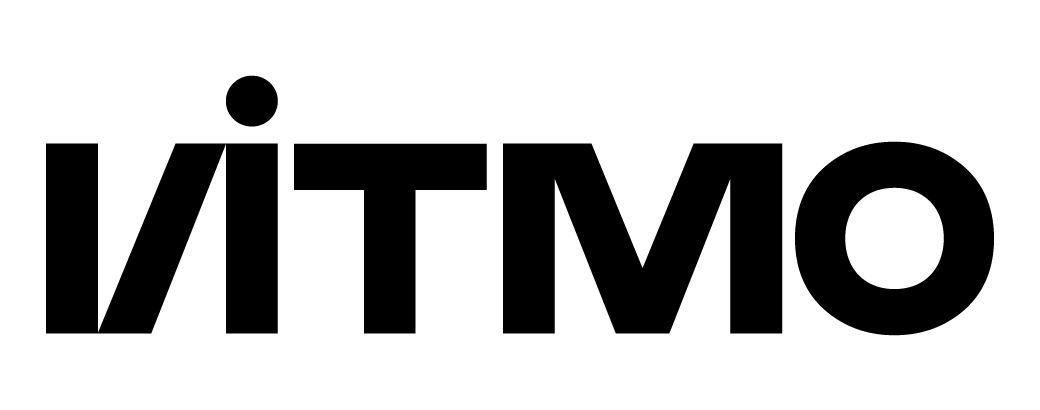
\includegraphics[width=4cm]{logo_itmo.png}\\[4mm]
    Санкт-Петербург, 2026\,г.
  \end{center}
\end{titlepage}

\section{Цель и задачи работы}

\textbf{Цель:} разработать систему управления доступом на микроконтроллере с клавиатурой, четырёхразрядным семисегментным индикатором и светодиодами.

\textbf{Задачи:}
\begin{enumerate}
  \item Организовать ввод четырёхзначного кода с мембранной клавиатуры.
  \item Отображать ввод на семисегментном индикаторе.
  \item Реализовать задание кода, закрытие сейфа и проверку кода для открытия.
  \item Отображать состояние сейфа светодиодами и сообщениями в консоли.
\end{enumerate}

\section{Схема взаимодействия процессора и периферийных устройств}

На рисунке~\ref{fig:seq} показана диаграмма последовательностей работы системы.

\begin{figure}[H]
  \centering
  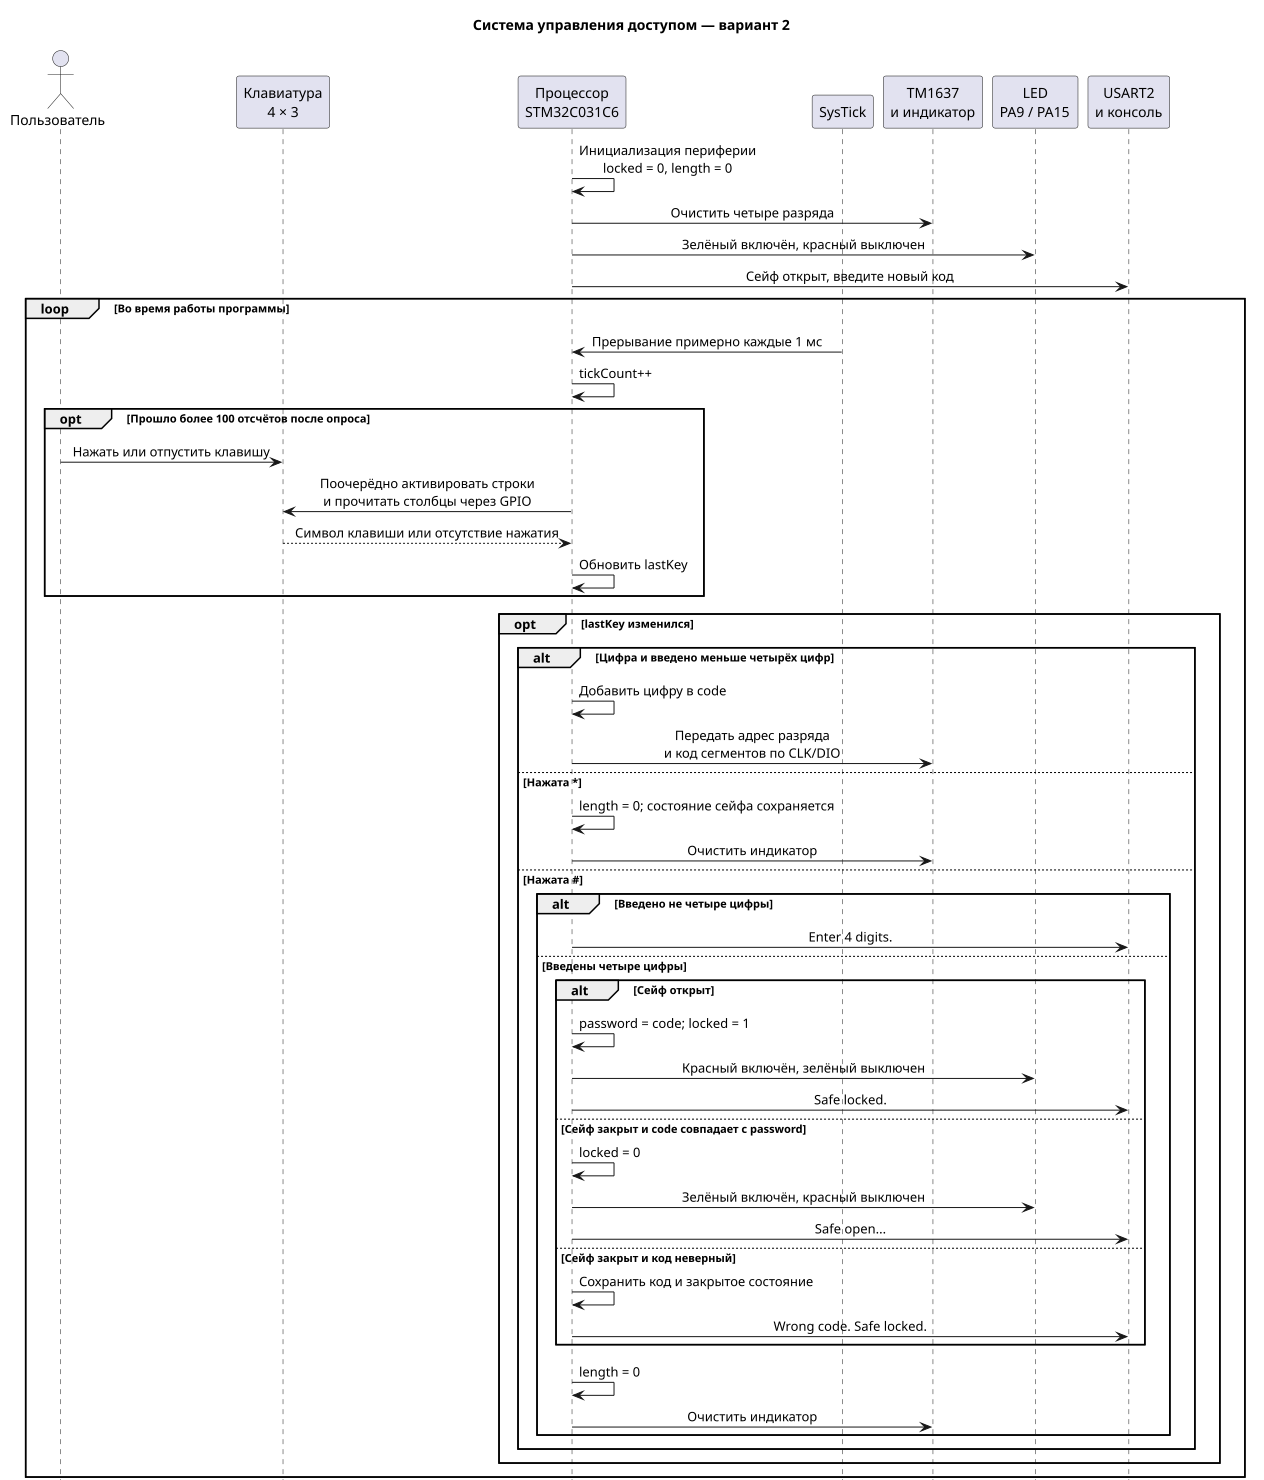
\includegraphics[width=\textwidth,height=.78\textheight,keepaspectratio]{sequence.png}
  \caption{Взаимодействие процессора, клавиатуры, индикатора и светодиодов}
  \label{fig:seq}
\end{figure}

\section{Описание процессов на схеме}

При запуске инициализируются GPIO, USART2, системный таймер SysTick, клавиатура и индикатор. Сейф открыт: включён зелёный светодиод. Сохранённый код и ввод хранятся в оперативной памяти.

Главный цикл периодически опрашивает строки и столбцы клавиатуры. Найденная клавиша преобразуется в символ. Каждая введённая цифра записывается в буфер и сразу отображается в соответствующем разряде индикатора. Начальные нули сохраняются.

В открытом состоянии ввод четырёх цифр и нажатие \texttt{\#} задают код и закрывают сейф. Включается красный светодиод. В закрытом состоянии такой же ввод проверяется: совпавший код открывает сейф и включает зелёный светодиод, несовпавший оставляет сейф закрытым. Результат выводится в последовательную консоль. После проверки ввод и индикатор очищаются.

Клавиша \texttt{*} очищает текущий ввод, не меняя состояние сейфа. Если нажать \texttt{\#} до ввода четырёх цифр, программа сообщает о неполном вводе. После открытия можно задать новый код. При перезапуске сейф открывается, код нужно задать заново.

\section{Руководство пользователя}

\begin{center}
  \begin{tabular}{ll}
    \toprule
    Клавиша или элемент & Назначение \\
    \midrule
    \texttt{0}--\texttt{9} & Ввод цифр \\
    \texttt{*} & Очистка текущего ввода \\
    \texttt{\#} & Задать код и закрыть либо проверить код \\
    Зелёный светодиод & Сейф открыт \\
    Красный светодиод & Сейф закрыт \\
    Индикатор & Показывает вводимые цифры \\
    \bottomrule
  \end{tabular}
\end{center}

Для закрытия сейфа введите четыре цифры и нажмите \texttt{\#}. Для открытия повторите ввод и подтвердите его клавишей \texttt{\#}. Клавиша \texttt{*} сбрасывает ввод.

\begin{figure}[H]
  \centering
  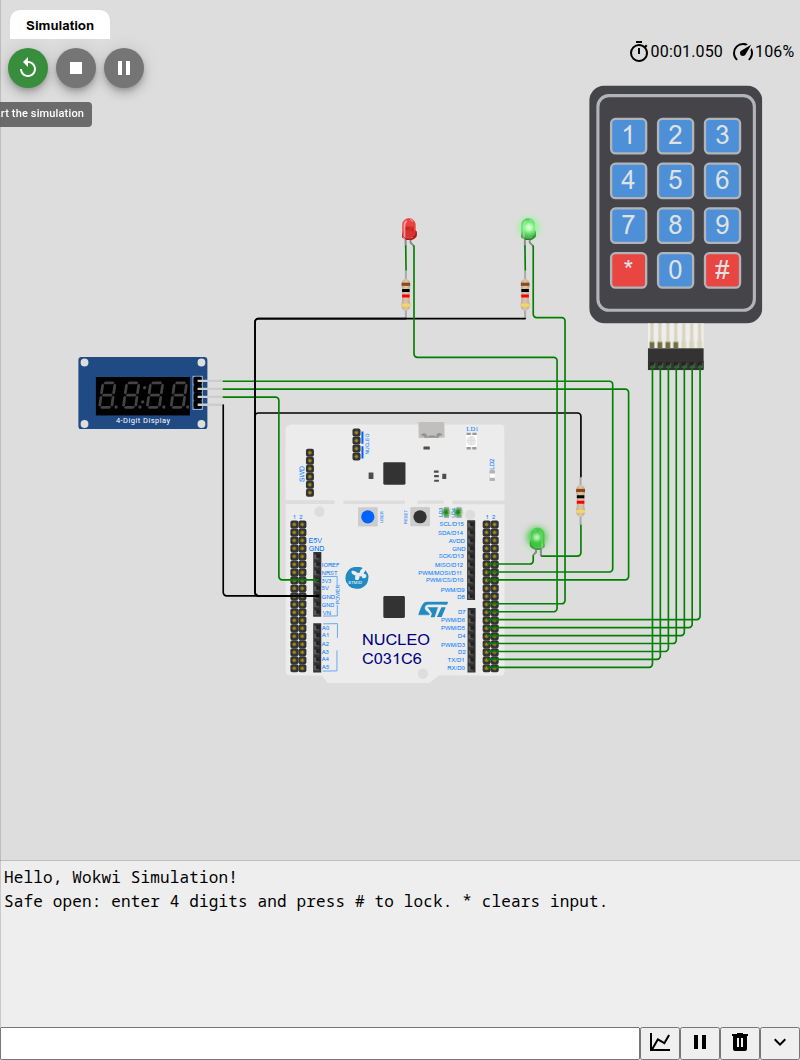
\includegraphics[width=.86\textwidth]{01-start.png}
  \caption{Начальное состояние: сейф открыт}
\end{figure}

\begin{figure}[H]
  \centering
  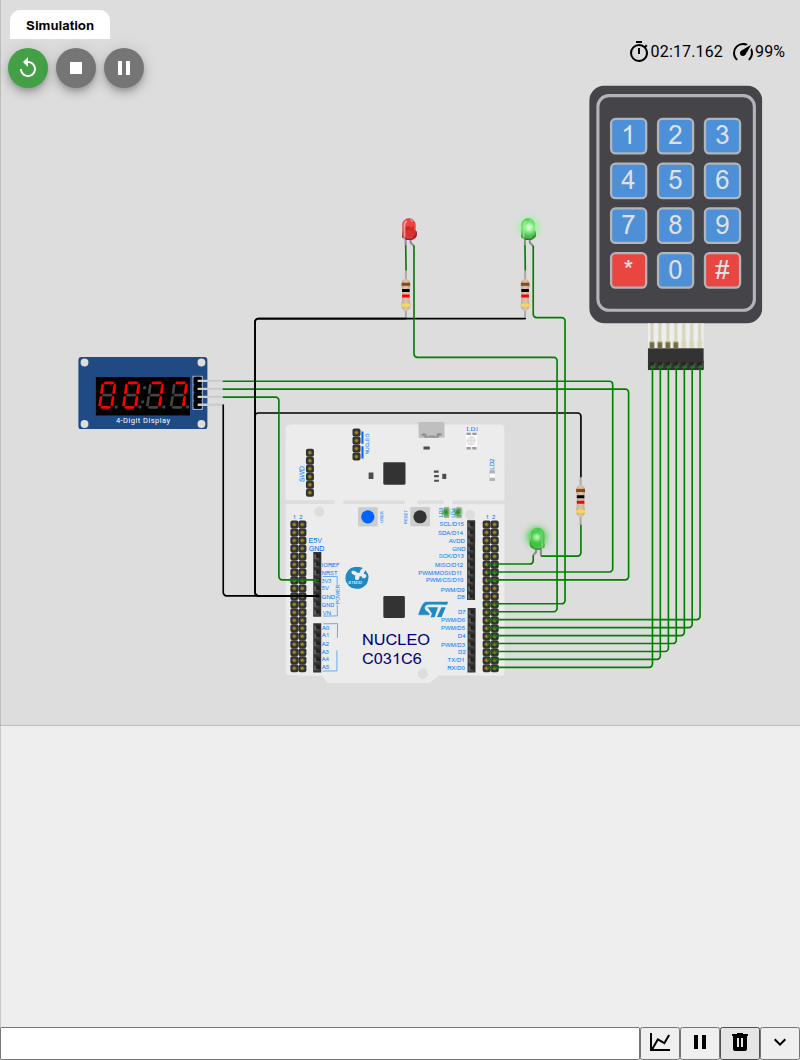
\includegraphics[width=.86\textwidth]{02-code.png}
  \caption{Ввод кода 0077}
\end{figure}

\begin{figure}[H]
  \centering
  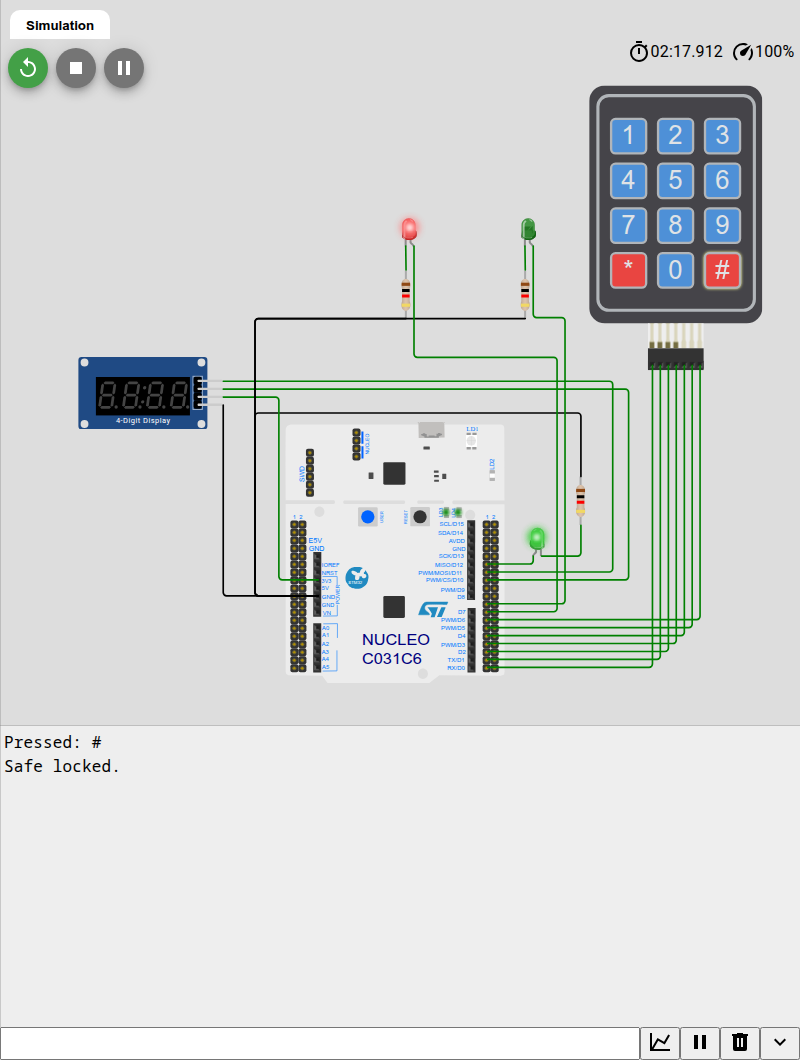
\includegraphics[width=.86\textwidth]{03-locked.png}
  \caption{Сейф закрыт}
\end{figure}

\begin{figure}[H]
  \centering
  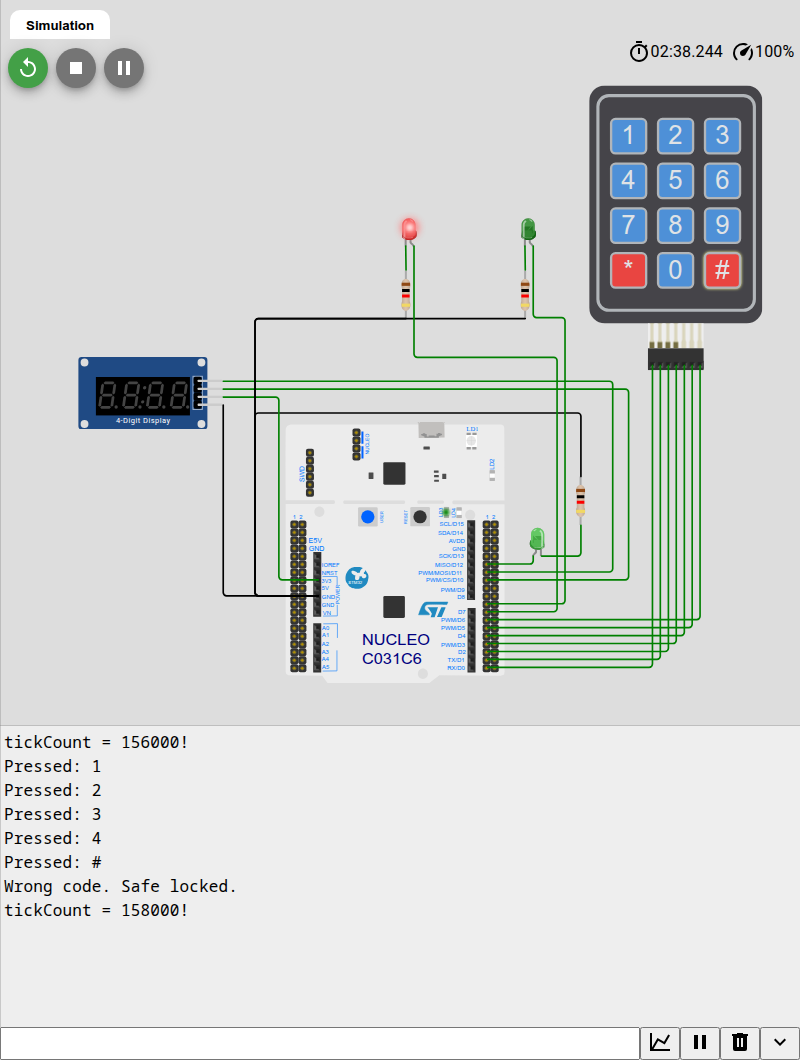
\includegraphics[width=.86\textwidth]{04-wrong.png}
  \caption{Отказ при неверном коде}
\end{figure}

\begin{figure}[H]
  \centering
  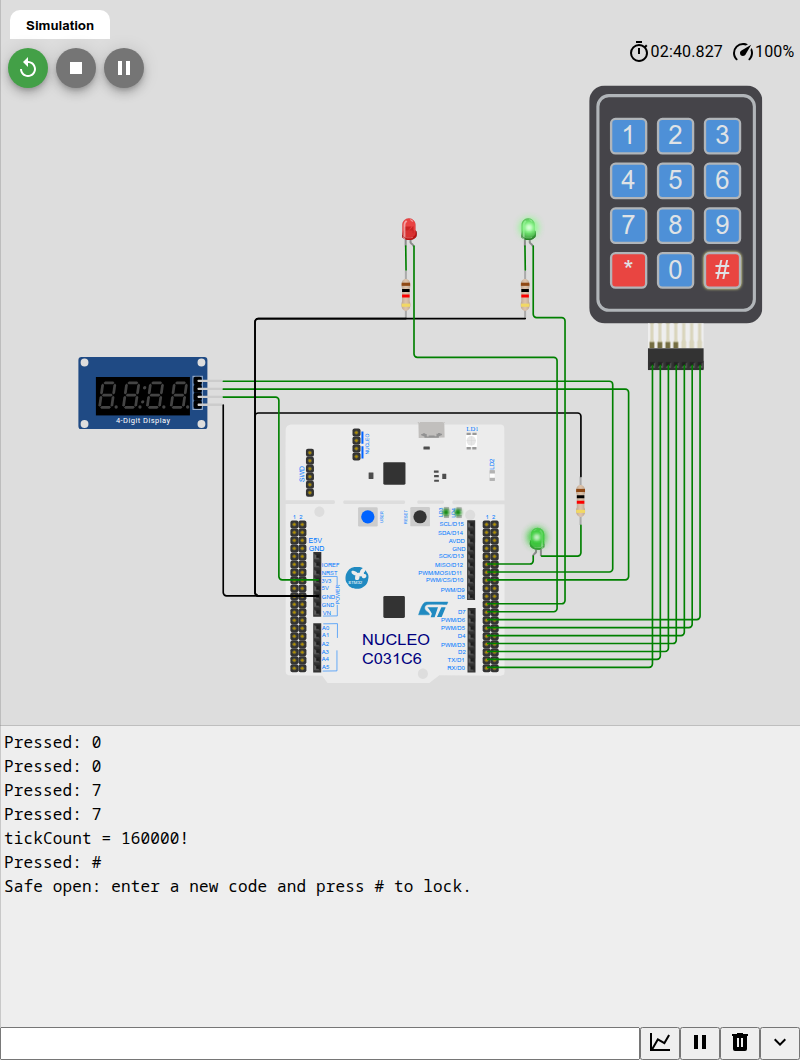
\includegraphics[width=.86\textwidth]{05-open.png}
  \caption{Открытие с правильным кодом}
\end{figure}

\begin{figure}[H]
  \centering
  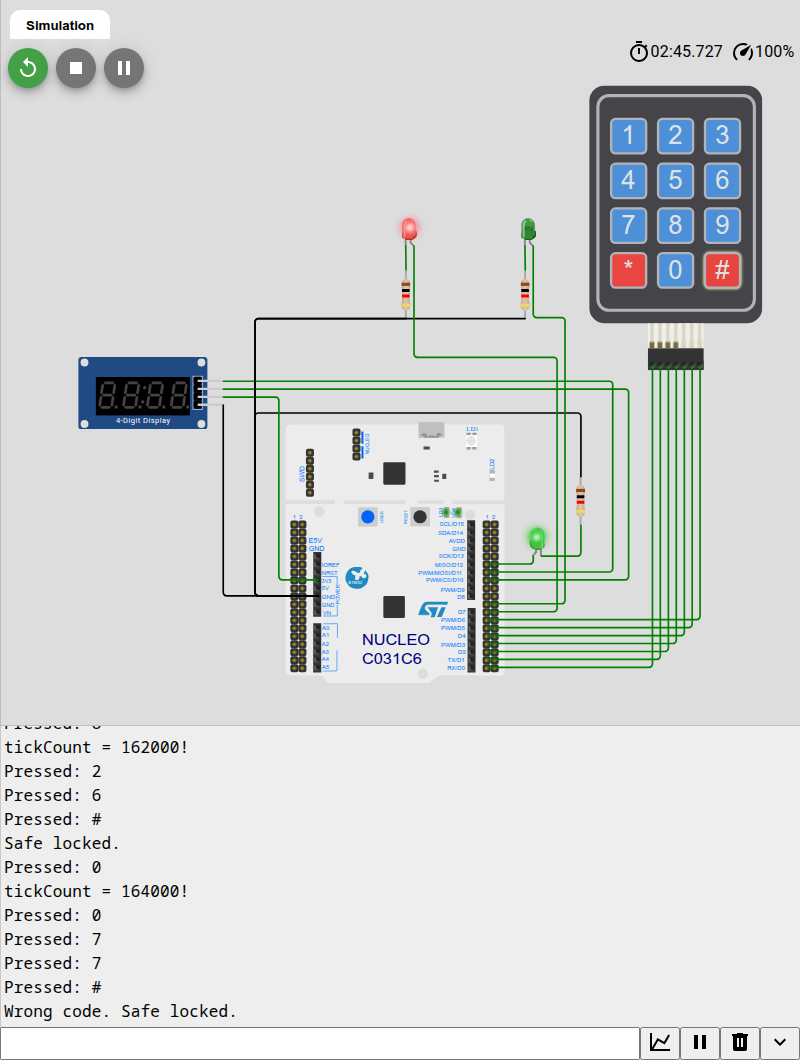
\includegraphics[width=.86\textwidth]{06-old-code.png}
  \caption{Старый код после смены отклоняется}
\end{figure}

\begin{figure}[H]
  \centering
  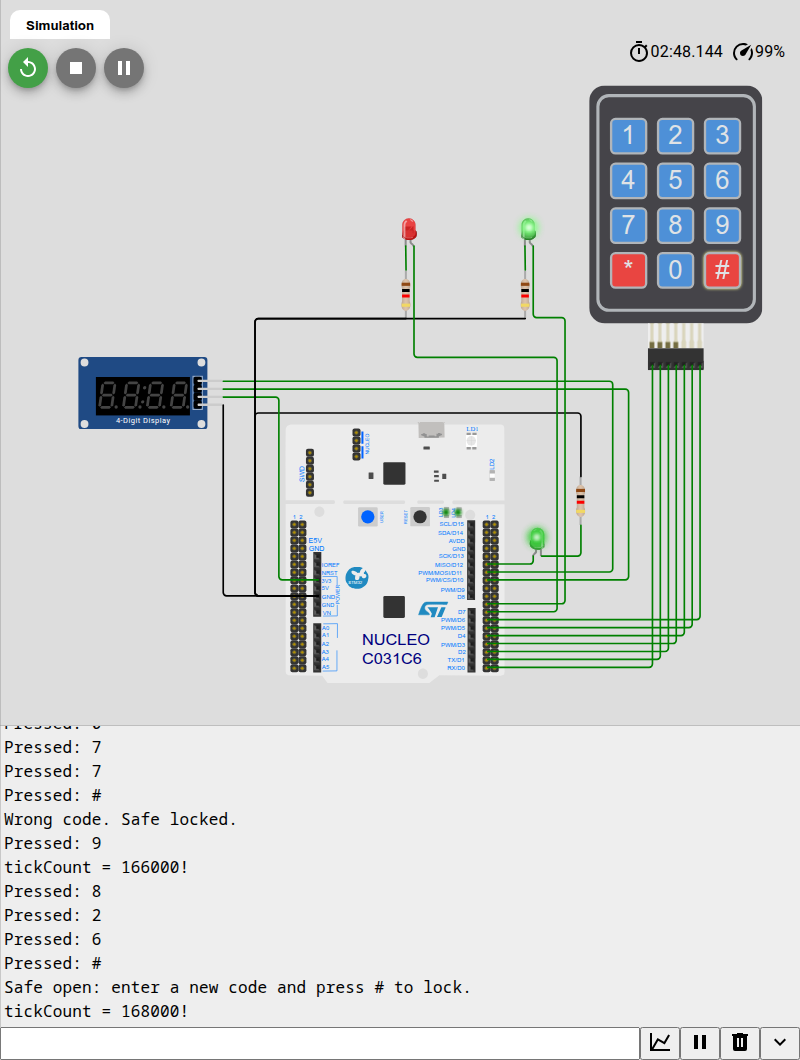
\includegraphics[width=.86\textwidth]{06-new-code.png}
  \caption{Открытие с новым кодом}
\end{figure}

\begin{figure}[H]
  \centering
  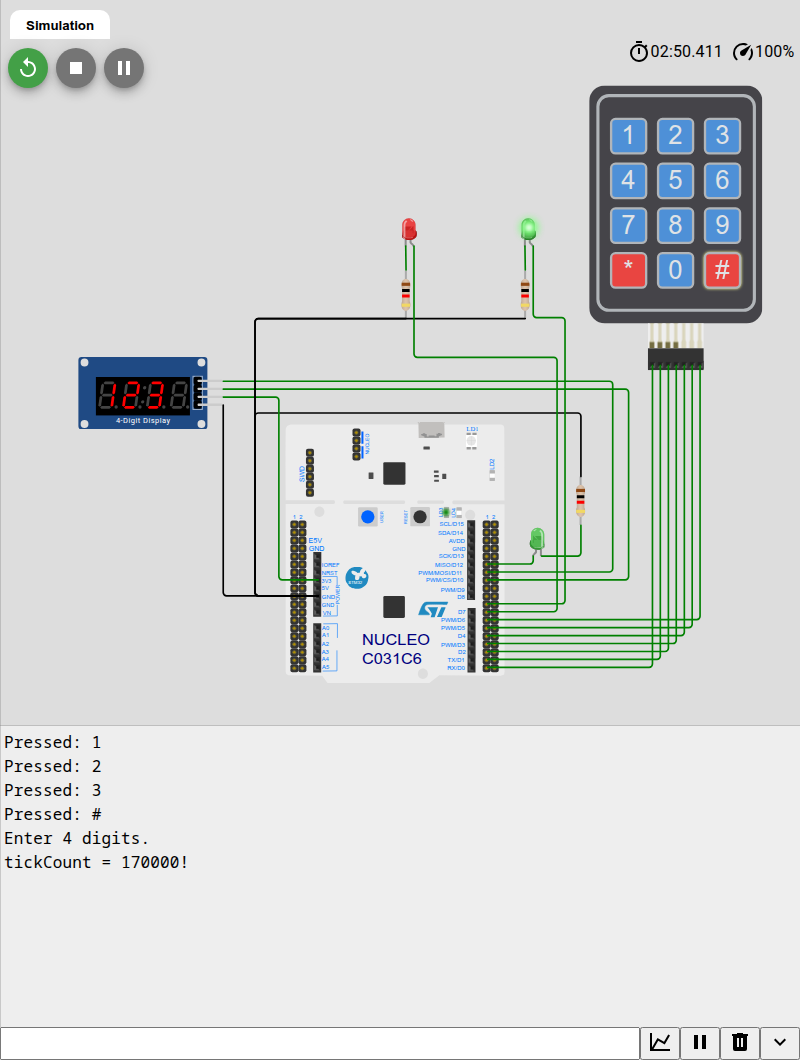
\includegraphics[width=.86\textwidth]{07-incomplete.png}
  \caption{Сообщение при неполном вводе}
\end{figure}

\section{Ссылка на репозиторий}

Исходный код: \url{https://github.com/pozitp/EmbeddedSystemMk1}.

\end{document}
